\textbf{{1. IPv4地址}}

把整个因特网看作一个单一的、抽象的网络。IP地址就是给每个连接在因特网上的主机(或路由器)分配一个在全世界范围是唯一的32位的标识符。一般将IP地址分为A类地址、B类地址、C类地址、D类地址和E类地址。D类地址为组播地址,将在IP组播中讲解,E类地址为保留地址,留作以后使用。

\textbf{{2.~}{A类地址}}

A类地址的网络号为\textbf{{前面8位,并且第一位规定为0}},如下图所示。

{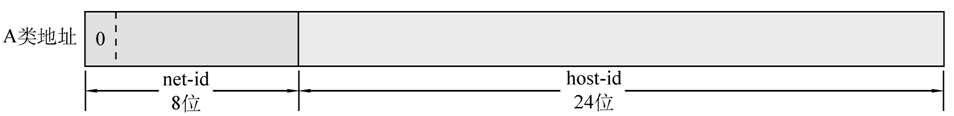
\includegraphics[width=2.70833in,height=0.33333in]{png-jpeg-pics/1A65DA1BD563DCDF16ECBAEF3C8B8C28.png}}

{{\textbf{A类地址可以指派的网络数为2}}\textsuperscript{{\textbf{7}}}{\textbf{-
2,}}{\textbf{\textbf{每个A类网络上的最大主机数是2}}}}\textsuperscript{{\textbf{24}}}{{\textbf{~-
2}}{\textbf{。}}}

{\textbf{{3. B}{类地址}}\\
}

{B类地址的网络号为\textbf{{前面16位,并且前面2位规定为10}},如下图所示。}

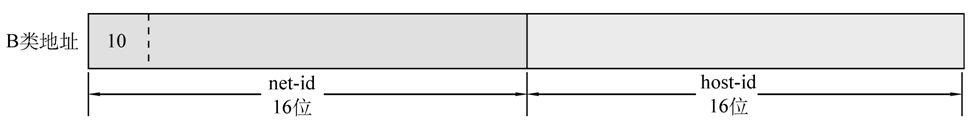
\includegraphics[width=3.12500in,height=0.40625in]{png-jpeg-pics/EA22F34752120C466F978054181B120D.png}

\textbf{{B类地址可以指派的网络数为2}\textsuperscript{{14}}{-1。每个B类网络上的最大主机数是2}\textsuperscript{{16}}{-2。}{}}

\textbf{\textbf{{4. C}{类地址}}\\
}

C类地址的网络号为\textbf{{前面24位,并且前面3位规定为110}},如下图所示。

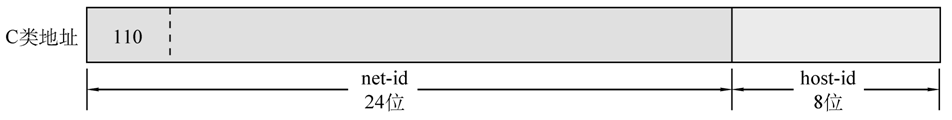
\includegraphics[width=3.12500in,height=0.39583in]{png-jpeg-pics/B14CB902462B4FC67C1283133496374C.png}

{\textbf{C类地址可以指派的网络数为2}}\textsuperscript{{\textbf{21}}}{\textbf{-1。\textbf{{每个C类网络上的最大主机数是}}2}}\textsuperscript{{\textbf{8}}}{\textbf{-2。}}

{\textbf{5. 六种特殊的IP地址}}

{\textbf{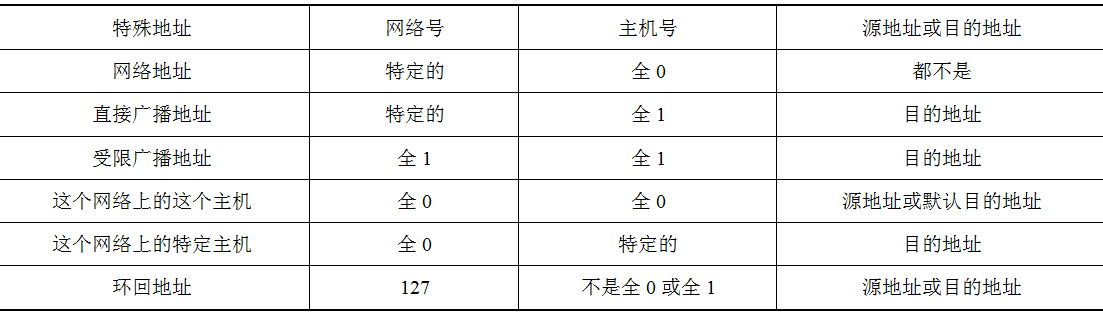
\includegraphics[width=3.33333in,height=0.94792in]{png-jpeg-pics/C5C2806E4ECEF23CF1FA33782EB94ECB.png}}}
